\documentclass[aspectratio=169]{../latex_main/tntbeamer}  % you can pass all options of the beamer class, e.g., 'handout' or 'aspectratio=43'
\usepackage{dsfont}
\usepackage{bm}
\usepackage[english]{babel}
\usepackage[T1]{fontenc}
%\usepackage[utf8]{inputenc}
\usepackage{graphicx}
\graphicspath{ {./figures/} }
\usepackage{algorithm}
\usepackage[ruled,vlined,algo2e,linesnumbered]{algorithm2e}
\usepackage{hyperref}
\usepackage{booktabs}
\usepackage{mathtools}

\usepackage{amsmath,amssymb}

\DeclareMathOperator*{\argmax}{arg\,max}
\DeclareMathOperator*{\argmin}{arg\,min}

\usepackage{amsbsy}
\newcommand{\vect}[1]{\bm{#1}}
%\newcommand{\vect}[1]{\boldsymbol{#1}}

\usepackage{pgfplots}
\pgfplotsset{compat=1.16}
\usepackage{tikz}
\usetikzlibrary{trees} 
\usetikzlibrary{shapes.geometric}
\usetikzlibrary{positioning,shapes,shadows,arrows,calc,mindmap}
\usetikzlibrary{positioning,fadings,through}
\usetikzlibrary{decorations.pathreplacing}
\usetikzlibrary{intersections}
\pgfdeclarelayer{background}
\pgfdeclarelayer{foreground}
\pgfsetlayers{background,main,foreground}
\tikzstyle{activity}=[rectangle, draw=black, rounded corners, text centered, text width=8em]
\tikzstyle{data}=[rectangle, draw=black, text centered, text width=8em]
\tikzstyle{myarrow}=[->, thick, draw=black]

% Define the layers to draw the diagram
\pgfdeclarelayer{background}
\pgfdeclarelayer{foreground}
\pgfsetlayers{background,main,foreground}

% Requires XeLaTeX or LuaLaTeX
%\usepackage{unicode-math}

\usepackage{fontspec}
%\setsansfont{Arial}
\setsansfont{RotisSansSerifStd}[ 
Path=../latex_main/fonts/,
Extension = .otf,
UprightFont = *-Regular,  % or *-Light
BoldFont = *-ExtraBold,  % or *-Bold
ItalicFont = *-Italic
]
\setmonofont{Cascadia Mono}[
Scale=0.8
]

% scale factor adapted; mathrm font added (Benjamin Spitschan @TNT, 2021-06-01)
%\setmathfont[Scale=1.05]{Libertinus Math}
%\setmathrm[Scale=1.05]{Libertinus Math}

% other available math fonts are (not exhaustive)
% Latin Modern Math
% XITS Math
% Libertinus Math
% Asana Math
% Fira Math
% TeX Gyre Pagella Math
% TeX Gyre Bonum Math
% TeX Gyre Schola Math
% TeX Gyre Termes Math

% Literature References
\newcommand{\lit}[2]{\href{#2}{\footnotesize\color{black!60}[#1]}}

%%% Beamer Customization
%----------------------------------------------------------------------
% (Don't) Show sections in frame header. Options: 'sections', 'sections light', empty
\setbeamertemplate{headline}{empty}

% Add header logo for normal frames
\setheaderimage{
	% 
\includegraphics[height=\logoheight]{figures/TNT_darkv4.pdf}
	
\includegraphics[height=\logoheight]{../latex_main/figures/luh_logo_rgb_0_80_155.pdf}
	% 
\includegraphics[height=\logoheight]{figures/logo_tntluh.pdf}
}

% Header logo for title page
\settitleheaderimage{
	% 
\includegraphics[height=\logoheight]{figures/TNT_darkv4.pdf}
	
\includegraphics[height=\logoheight]{../latex_main/figures/luh_logo_rgb_0_80_155.pdf}
	% 
\includegraphics[height=\logoheight]{figures/logo_tntluh.pdf}
}

% Title page: tntdefault 
\setbeamertemplate{title page}[tntdefault]  % or luhstyle
% Add optional title image here
%\addtitlepageimagedefault{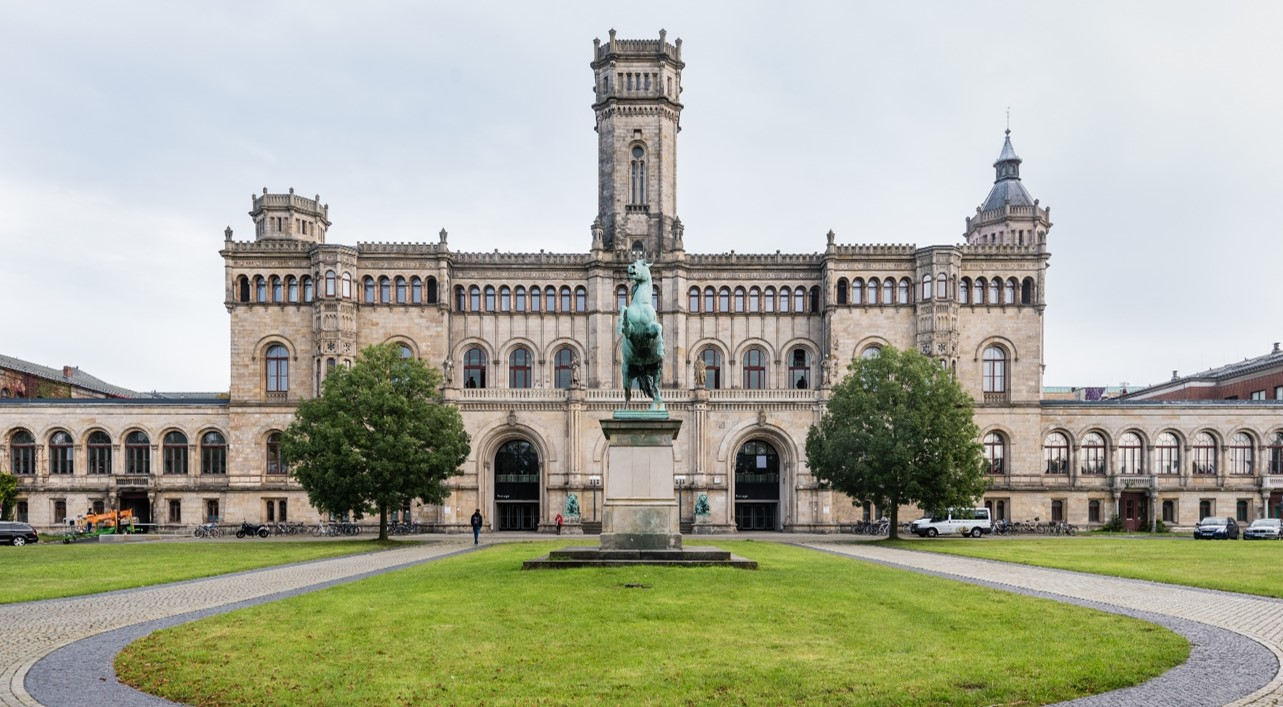
\includegraphics[width=0.65\textwidth]{figures/luh_default_presentation_title_image.jpg}}

% Title page: luhstyle
% \setbeamertemplate{title page}[luhstyle]
% % Add optional title image here
% \addtitlepageimage{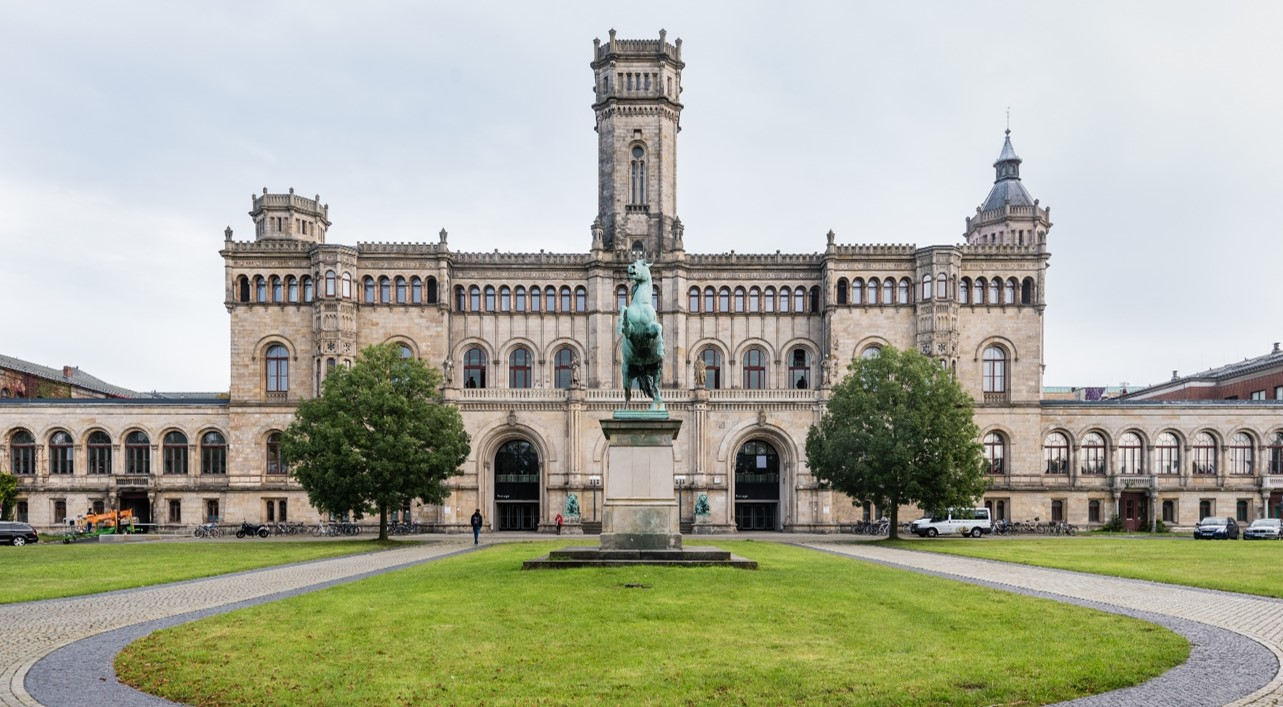
\includegraphics[width=0.75\textwidth]{figures/luh_default_presentation_title_image.jpg}}

\author[Abedjan \& Lindauer]{Ziawasch Abedjan \& Marius Lindauer\\[1em]
	
\includegraphics[height=\logoheight]{../latex_main/figures/luh_logo_rgb_0_80_155.pdf}\qquad
	
\includegraphics[height=\logoheight]{../latex_main/figures/DBIS_Kurzlogo.png}\qquad

\includegraphics[height=\logoheight]{../latex_main/figures/TNT_darkv4}\qquad

\includegraphics[height=\logoheight]{../latex_main/figures/L3S.jpg}	}
\date{Summer Term 2022; \hspace{0.5em} {
\includegraphics[height=1.5em]{../latex_main/figures/Cc-by-nc-sa_icon.svg.png}}; based on \href{https://ds100.org/fa21/}{[DS100]}
}


%%% Custom Packages
%----------------------------------------------------------------------
% Create dummy content
\usepackage{blindtext}

% Adds a frame with the current page layout. Just call \layout inside of a frame.
\usepackage{layout}


%%% Macros
%\renewcommand{\vec}[1]{\mathbf{#1}}
% \usepackage{bm}
%\let\vecb\bm

\title[Introduction]{DS: Clustering, Part 1}
\subtitle{Minimizing Inertia}

\graphicspath{ {./figure/} }
%\institute{}


\begin{document}
	
	\maketitle
	\begin{frame}{K-Means Clustering for K = 4}
	    Below is an example of an output for K=4:
	    \begin{figure}
	        \centering
	        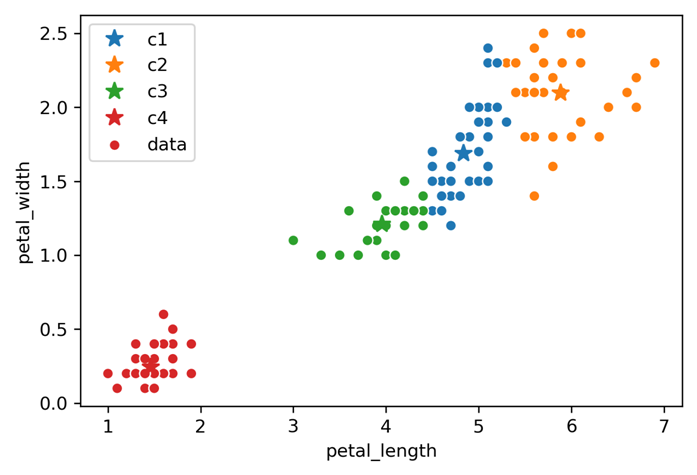
\includegraphics[scale=.75]{Bild21}
	    \end{figure}
	\end{frame}
	
	
	\begin{frame}{K-Means Clustering for K = 4}
	    Each time you run K-Means, you get a different output
	    \begin{figure}
	        \centering
	        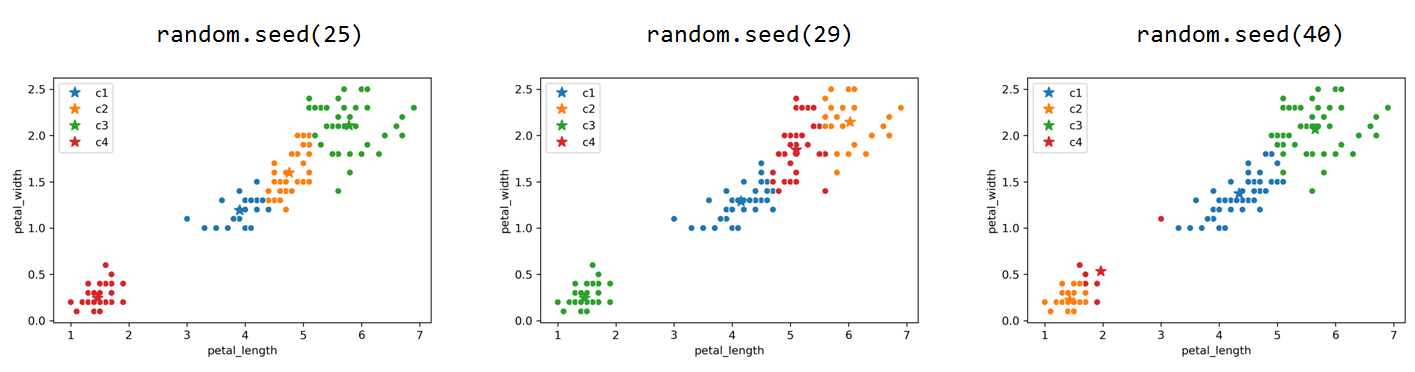
\includegraphics[scale=.4]{Bild22}
	    \end{figure}
	    Which is best?
	    \begin{itemize}
	        \item One approach: Define some sort of loss function
	        \pause
	        \item Come up with a loss function for clustering
	    \end{itemize}
	\end{frame}
	
	
	\begin{frame}{K-Means Clustering for K = 4}
	    Each time you run K-Means, you get a different output
	    \begin{figure}
	        \centering
	        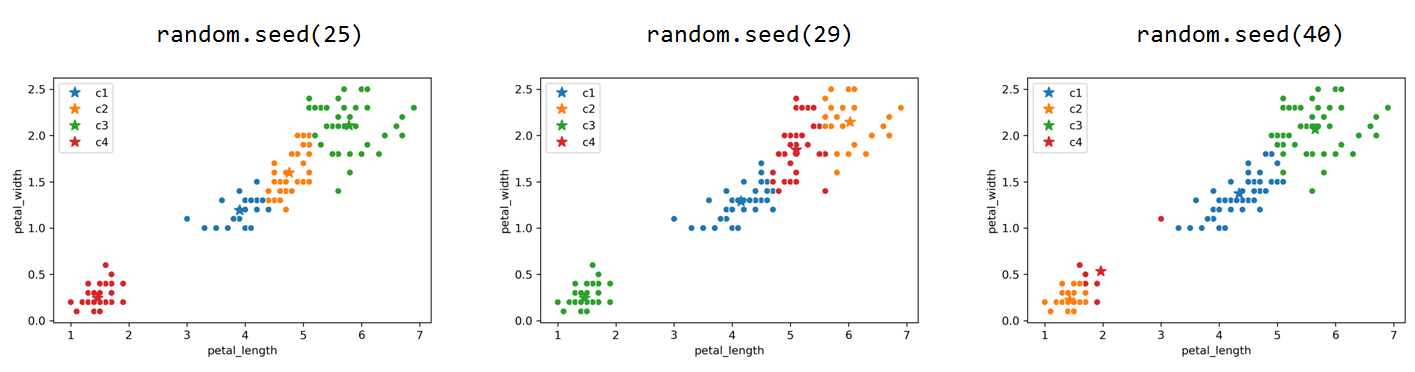
\includegraphics[scale=.4]{Bild22}
	    \end{figure}
	    Come up with a loss function for clustering -- your ideas:
	    \begin{itemize}
	        \item The sum of distances from each point to its center
	        \item Could take into account balance of number of points per cluster
	    \end{itemize}
	\end{frame}
	
	
	\begin{frame}{K-Means Clustering for K = 4}
	    To evaluate different clustering results, we need a loss function
	    \begin{columns}
	        \begin{column}{.5\textwidth}
	                \begin{figure}
	                    \centering
	                    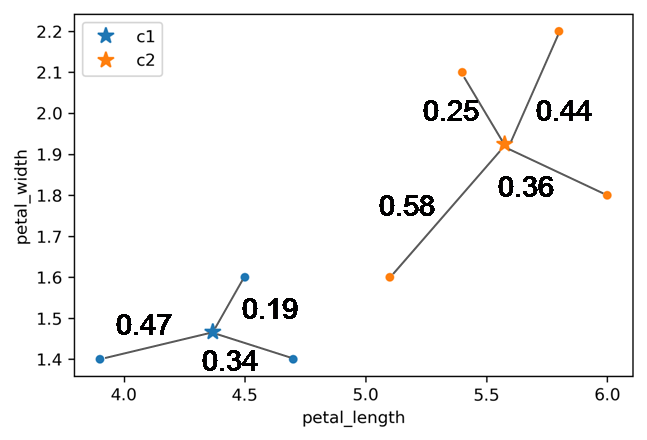
\includegraphics[scale=.5]{Bild23}
	                \end{figure}
	        \end{column}
	        
	        \begin{column}{.5\textwidth}
	                Two common loss functions:
	                \begin{itemize}
	                    \item Inertia: Sum of squared distances from each data point to its center
	                    \item Distortion: Weighted sum of squared distances from each data point to its center
	                \end{itemize}
	                Example: 
	                \begin{itemize}
	                    \item Inertia: 0.47$^2$ + 0.19$^2$ + 0.34$^2$   + 0.25$^2$ + 0.58$^2$ + 0.36$^2$ + 0.44$^2$
	                    \item Distortion: (0.47$^2$ + 0.19$^2$ + 0.34$^2$)/3 + (0.25$^2$ + 0.58$^2$ + 0.36$^2$ + 0.44$^2$)/4

	                \end{itemize}
	        \end{column}
	    \end{columns}
	\end{frame}
	
	
	
	\begin{frame}{K-Means Clustering for K = 4}
	    Each time you run K-Means, you get a different output
	    \begin{figure}
	        \centering
	        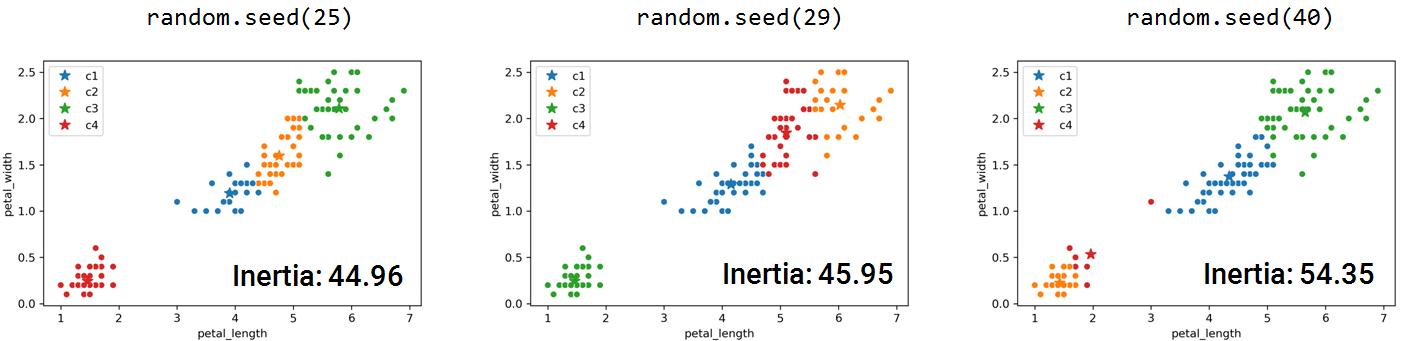
\includegraphics[scale=.4]{Bild24}
	    \end{figure}
	   Our loss function says that the leftmost clustering is best (inertia: 44.96) and rightmost clustering (inertia: 54.35) is worst

	\end{frame}
	
	
	\begin{frame}{K-Means and Inertia}
	    It turns out that the function K-Means is trying to minimize is inertia\\
… but often fails to find global optimum. Why?\\
Can think of K-means as a pair of optimizers that take turns
    \begin{itemize}
        \item First optimizer:
        \begin{itemize}
            \item Holds center positions constant
            \item Optimizes data colors
        \end{itemize}
        \item Second optimizer:
        \begin{itemize}
            \item Holds data colors constant
            \item Optimizes center positions
        \end{itemize}
        \item Neither gets total control 
    \end{itemize}
	\end{frame}
	
	
	
	\begin{frame}{Optimizing Inertia}
	    Hard problem: Give an algorithm that optimizes inertia
	    \begin{itemize}
	        \item Your algorithm should return the EXACT best centers and colors
	        \item Don’t worry about runtime
	    \end{itemize}
	    This is a bit of a CS61B/CS70/CS170 problem. It may be far too hard for some of you.
	\end{frame}
	
	
	\begin{frame}{Optimizing Inertia}
	    Hard problem: Give an algorithm that optimizes inertia
	    \begin{itemize}
	        \item Your algorithm should return the EXACT best centers and colors
	        \item Don’t worry about runtime
	    \end{itemize}
	    Algorithm:
	    \begin{itemize}
	        \item For all possible kn colorings:$\leftarrow$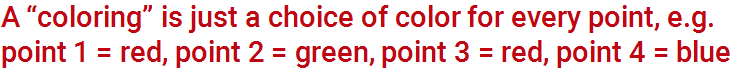
\includegraphics[scale=.35]{Bild25}
	        \begin{itemize}
	            \item Compute the k centers for that coloring
	            \item Compute the inertia for the k centers
	            \begin{itemize}
	                \item If current inertia is better than best known, write down the current centers and coloring and call that the new best known
	            \end{itemize}
	        \end{itemize}
	    \end{itemize}
	    No better algorithm has been found$\leftarrow$
\includegraphics[scale=.35]{Bild26}
	    %\bigskip
	    %*A “coloring” is just a choice of color for every point, e.g. point 1 = red, point 2 = green, point 3 = red, point 4 = blue\\
	    %**For those who know what this means: K-Means is known to be an NP-hard problem
	    
	\end{frame}
	
	
\end{document}